\chapter{Funcionamento Geral}

\section{Sensores}
\par Os sensores analógicos enviam ao microcontrolador, Arduino due, sinais analógicos que são variações de tensão entre 0V a 5V, em que essa variação ocorre de acordo com o que o sensores está captando, por meio da variação da capacitância, indutância ou da resistividade, em que a frequência de discretização do sinal não ultrapasse  seja de no máximo 2 MHz. Os sensores digitais enviam sinais de ondas quadradas, com frequência máxima 2 MHz, com níveis lógicos 0V e 5V. São eles:
\par \textbf{Sensores analógicos:}
    \begin{itemize}
        \item Sensor de umidade e temperatura: modelo DHT11;
        \item Sensor de fumaça e gases tóxicos: modelo MQ-2.
    \end{itemize}
\par \textbf{Sensores analógicos:}
    \begin{itemize}
        \item Sensor de presença, modelo: Qualitronix QA25.
    \end{itemize}

\subsection{Exemplo do Funcionamento do Sensor}

\begin{figure}[!h]
\caption{Funcionamento do Sensor}
\centering
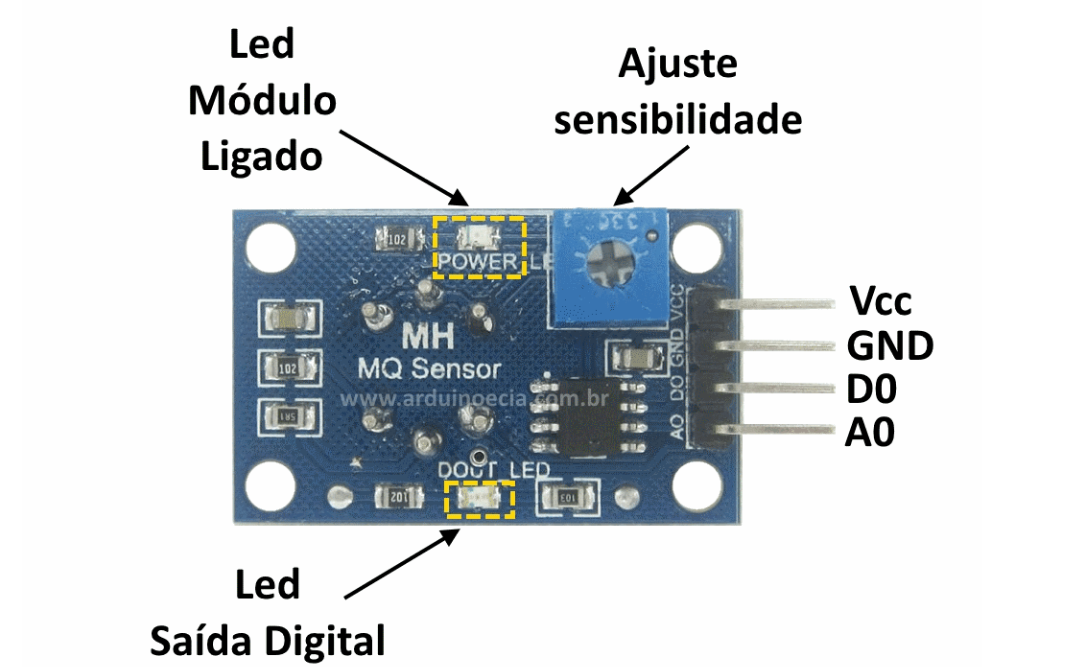
\includegraphics[width=10cm]{figuras/funcionamento}
\end{figure}

\par O sensor MQ-2 (datasheet), é um detector de gás e fumaça que pode indicar a presença de GLP (Gás liquefeito de petróleo, o famoso gás de cozinha), Propano, Metano, Hidrogênio e outros tipos de gases. Seu nível de detecção vai de 300 a 10.000 ppm (partes por milhão), ajustáveis por um potenciômetro na parte de trás do módulo. Um chip comparador LM393 é responsável por ler as informações do sensor e converter essas informações em sinais para o microcontrolador.
\par A tensão de alimentação do módulo é de 5V e a comunicação com o microcontrolador pode ser feita de duas maneiras : pela saída digital D0 ou pela saída analógica A0. Podemos utilizar a saída digital para simplesmente ligar uma sirene ou acionar um relé que vai fechar/abrir uma porta, cortar o fornecimento de gás, etc. Já a saída analógica informa o nível de concentração de gases detectados pelo sensor. Quanto maior a concentração, maior o nível de sinal na saída analógica A0.

\begin{figure}[!h]
\caption{Esquemático do Funcionamento do Sensor}
\centering
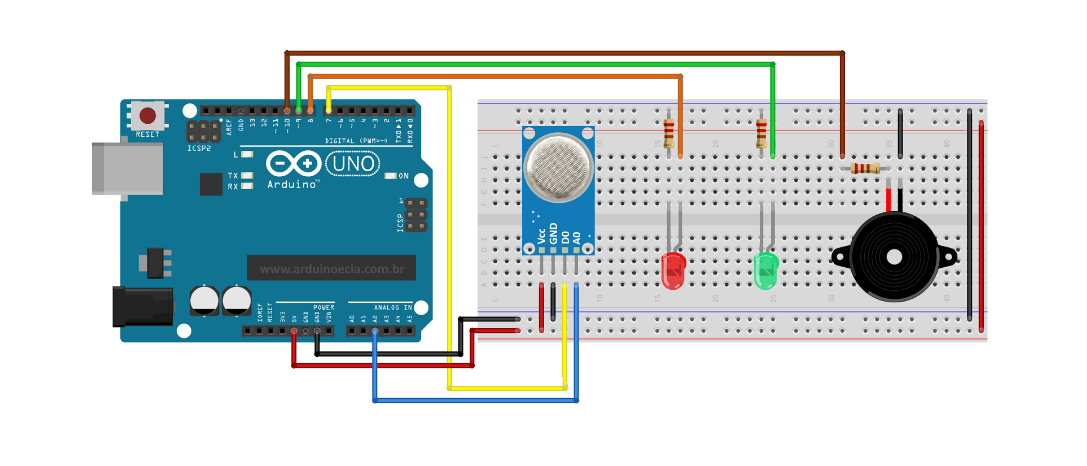
\includegraphics[width=10cm]{figuras/funcionamento2}
\end{figure}

\par A exemplo de outros sensores para Arduino, vamos trabalhar apenas com portas digitais e analógicas, lendo os valores enviados pelo sensor. No nosso circuito de testes, usamos a porta digital 7 para ligação ao pino D0 do módulo, e a porta analógica A2 ligada ao pino A0 do módulo.
\par As portas digitais 8, 9 e 10 serão utilizadas para acionar um led vermelho e um buzzer (gás detectado), e um led verde no modo normal de operação (sem alarme).
\par No programa, o valor lido da porta analógica (valor\_analogico), é comparado com a variável nivel\_sensor para determinar em que ponto será acionado o buzzer e a também o led vermelho.
\par Nos nossos testes, o valor inicial da leitura ficou em 213, e aumentou rapidamente para 550 na presença de gás. Ajuste o valor de nivel\_sensor de acordo com o nível de detecção desejado.
\par O código-fonte da programação deste sistema encontra-se nos anexos deste documento.

\section{Atuadores}
\par Os atuadores são todos aparelhos que dependem do sistema para serem ativados ou desativados, de forma lógica, em que para serem ativados, o nível lógico será de 0V, que no caso é 0, para serem ativados, o nível lógico é de 5V. Para a centra, que funciona com 5V contínuo (DC), poder controlar os eletrodomésticos da casa que funcionam com 220V alternada (AC), são utilizados relés, que são chaves automáticas acionadas com 5V DC para fechar ou abrir o circuito de 220 AC.

\section{Sensores Botões}
\par Estes sensores enviam dois níveis lógicos, 0V ou 5V que representam se o botão está apertado ou não. Estes sensores são as tomadas para ligar e desligar a  luz do cômodo da casa, como um opção para o usuário para não depender somente da plataforma para esta função.

\section{Arduino}
\par O Arduino é responsável por receber os sinais dos sensores analoógicos, por causa do seu conversor AD que está embutido, e digitais e tratar as informações dos sinais para que obter os parâmetros que representam o que os sensores estão lendo.
\par A segunda função é dar os comando para os relés para poder ligar ou desligar, conforme receber comandos da central ou dos botões presentes nos cômodos. A central envia comando via serial, por conexão USB, usando o protocolo da IDE do Arduino, para o arduino dar comandos aos seus atuadores.
\par A terceira função do Arduino é enviar os parâmetros dos sensores já tratados e o estado dos atuadores, entre ligado e desligados, via serial, por conexão USB, usando o protocolo da IDE do Arduino.
\par A informações trocadas trocadas senão strings com códigos de comando e parâmetros, de forma que os programas no Arduino e na central, Raspberry entendam.
\par A linguagem de programação do Arduino é em C++ e Assembler, com funções e bibliotecas exclusivas para a arquitetura do Arduino .

\section{Central}
\par A central é composta por uma Raspberry, com função de integrar o sistemas inteiro. Além de se comunicar com o Arduino, enviando comandos e remendos parâmetros via serial USB, a Raspberry se comunica com o sistema de smart grid via serial USB, com as câmeras de vigilância dia wifi, com o Hard Disk para armazenamento e dados via serial USB e da plataforma via internet por SSH.
\par O sistema operacional da central é uma versão do Linux para Raspberry, que o Raspbian, arquitetura 32bits. No sistema, está instalado os programas para o funcionamento do sistemas para integrar todos os outros blocos, armazenado e lendo todos os dados obtidos dos outros blocos necessário no HD.

\section{Comunicação}
\par As setas ‘A’ e ‘C’ indicam que os sensores e os botões, que também são sensores, apenas enviaram informações, sinais. Para o sensores analogicos será um sinal contínuo no tempo variando a tensão entre 0V e 5V, pois a alimentação desses sensores é de 5V e suas saídas são de até 5V, neles já estão integrados o circuito de offset de 2,5V, pois o Arduino não trabalha com tensões negativas, e também estão integrados o amplificadores operacionais, para  amplificar o sinal que realmente sai do sensor, pois as variações de tensão são muito pequenas para que o Arduino possa captar.
\par Na leitura dos sensores analógicos, a frequência para discretização do sinal deve ser de no mínimo 2 vezes a frequência do sinal e essa frequência de discretização pode ser de no máximo 2MHz. Concorrer distorções de leitura do sinal analógico caso ultrapasse esse limite, pois ocorrerá sobreposição na discretização do sinal, perdendo informações.
\par No Arduino, em suas portas analógiras, para cada uma das portas há um conversor AD, convertendo o sinal para um sinal de função degrau, isso ocorre internamente no arduino e também já tem bibliotecas prontas, específicas para cada sensor analógico, que são responsáveis por interpretar esses sinais e apresentar para o programador um valor compreensível.Para os sensores digitais, o  tipo de sinal que eles enviam é apenas  níveis lógicos 0V e 5V, como estado verdadeiro ou falso de um sensor, em que ao longo do tempo forma-se uma onda quadrada, ou pode ser um sinal de função escada, em que há níveis de tensão definidos, com 8 degraus, ou seja, 8 níveis de tensão fixos entre 0V e 5V, a frequência dos sinais digitais não podem passar de 2MHz também. A conexão dos sensor para o arduino será por meio de cabo axial, porque esse tipo de cabo conte blindagem eletromagnética, o que evita ruído por interferência de sinais externos indesejados e ruídos provocados por cabos inadequados.
\par Na seta ‘B’, os atuadores recebem, no caso do projeto deste quite, apenas comandos em níveis lógicos, verdadeiro ou falso, que são respetivamente 0V e 5V. Desta forma se controla relés que são acionados com 5V e desativados com 0V, em que, respectivamente, ativa e desativa os aparelhos conectados, em que funcionam com 220V AC.
\par As setas ‘D’ é a comunicação entre o Arduino e a Raspberry, que é por serial USB, usando o protocolo de dados é definido pela IDE do Arduino, que está instalada na Raspberry. Essa comunicação é uma via de mão dupla, em que as informações são transmitidas em uma sequência de valores em binário.

\begin{center}
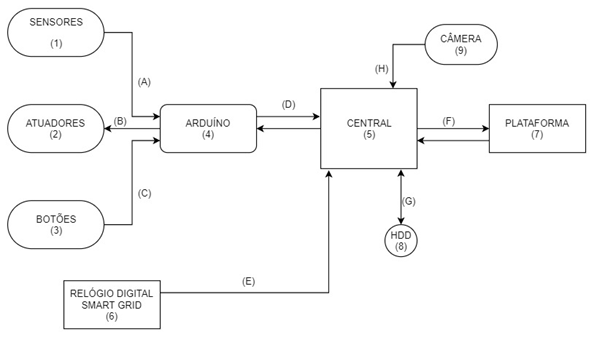
\includegraphics[width=\textwidth]{figuras/blocoskit}
\end{center}
